\section{実験}

前節で説明した方法により,15種類のNタプルネットワークのそれぞれについて,Optimistic initialization の初期値 $\mathit{OI}$ を3通り変えて学習を行った.
ランダム性の影響を抑えるため,各条件について乱数のシードを変えて10回の学習を行い,10個のNタプルネットワークを得た.
次に,各Nタプルネットワークに対し,GreedyプレイおよびExpectimax探索(深さ2〜6)により1000ゲームのプレイを行い,それらの平均スコアを求めた.
本節のグラフにおいて,10個のNタプルネットワークの平均を点や線で示し,それらの標準偏差をエラーバー等で示す.

% 本研究では,ミニ2048におけるNタプルネットワークの学習性能を多角的に分析するため,
% 構造の異なる複数のプレイヤを構築し,GreedyおよびExpectimax探索による評価を行った.

% \ref{tuples}で示した15種類のプレイヤを用いて評価を行った.

% さらに,Optimistic Initialization(OI)の影響を調べるため,
% 各プレイヤについてOIの初期値を0,1200,5400に設定し,それぞれ学習を実施した.
% すべてのプレイヤは $5 \times 10^8$ 手分の行動に基づいて学習を行い,
% 乱数シードを変えて10体ずつ学習させた.結果として,
% $15$タプル構成$\times 3$回(OIの初期値)$\times 10$回(シード)で,計$450$体のプレイヤが作成された.

% これらのプレイヤに対して,1000ゲームプレイを行い,
% seed違いの結果をまとめた10000ゲームのログを用いて解析を行なった.

\subsection{スコアとパラメータ数の関係}
第1節で示した RQ1 について考察するため,Greedy プレイのスコアを,Optimistic initialization の初期値($\mathit{OI}$)ごとにプロットしたものが図\ref{fig:score_vs_tuple_OI0}から図\ref{fig:score_vs_tuple_OI5400}である.これらのグラフは,横軸にパラメータ数の対数をとり,縦軸にスコアの平均値と標準偏差をプロットしている.また,それぞれのグラフの点に対し,パラメータ数の対数とスコアの関係を二次関数でフィッティングして得られる近似曲線も描いている.

これらのグラフから,いずれのグラフもおよそ放物線を描いていることが分かる.
とくに,\textsf{5M}から\textsf{6F}の区間に放物線の頂点が位置することが確認できた.
また,$\mathit{OI}=0$の場合(図\ref{fig:score_vs_tuple_OI0}),3種類の初期値の中で標準偏差が大きいものが目立っている.このことは,Optimistic initializationを行わない学習では,学習の幅広さが足りず,安定的に良い結果が得られないことを意味する.
$\mathit{OI}=1200$ と $\mathit{OI}=5400$の場合(図\ref{fig:score_vs_tuple_OI1200},図\ref{fig:score_vs_tuple_OI5400}),スコアのばらつきは小さい.
また,より多くのパラメータ数のところまでスコアの向上が見られる(すなわち,放物線の頂点が右に移動する).
\textsf{5F}よりもパラメータ数の少ないNタプルネットワークでは,平均スコアは初期値にそれほど依存していない.一方,それよりも多くのパラメータを持つNタプルネットワークでは,初期値が $\mathit{OI}=1200$ の場合に最も良い結果が得られた.

\begin{figure}[t]
    \centering
    \begin{subfigure}[b]{\linewidth}
        \centering
        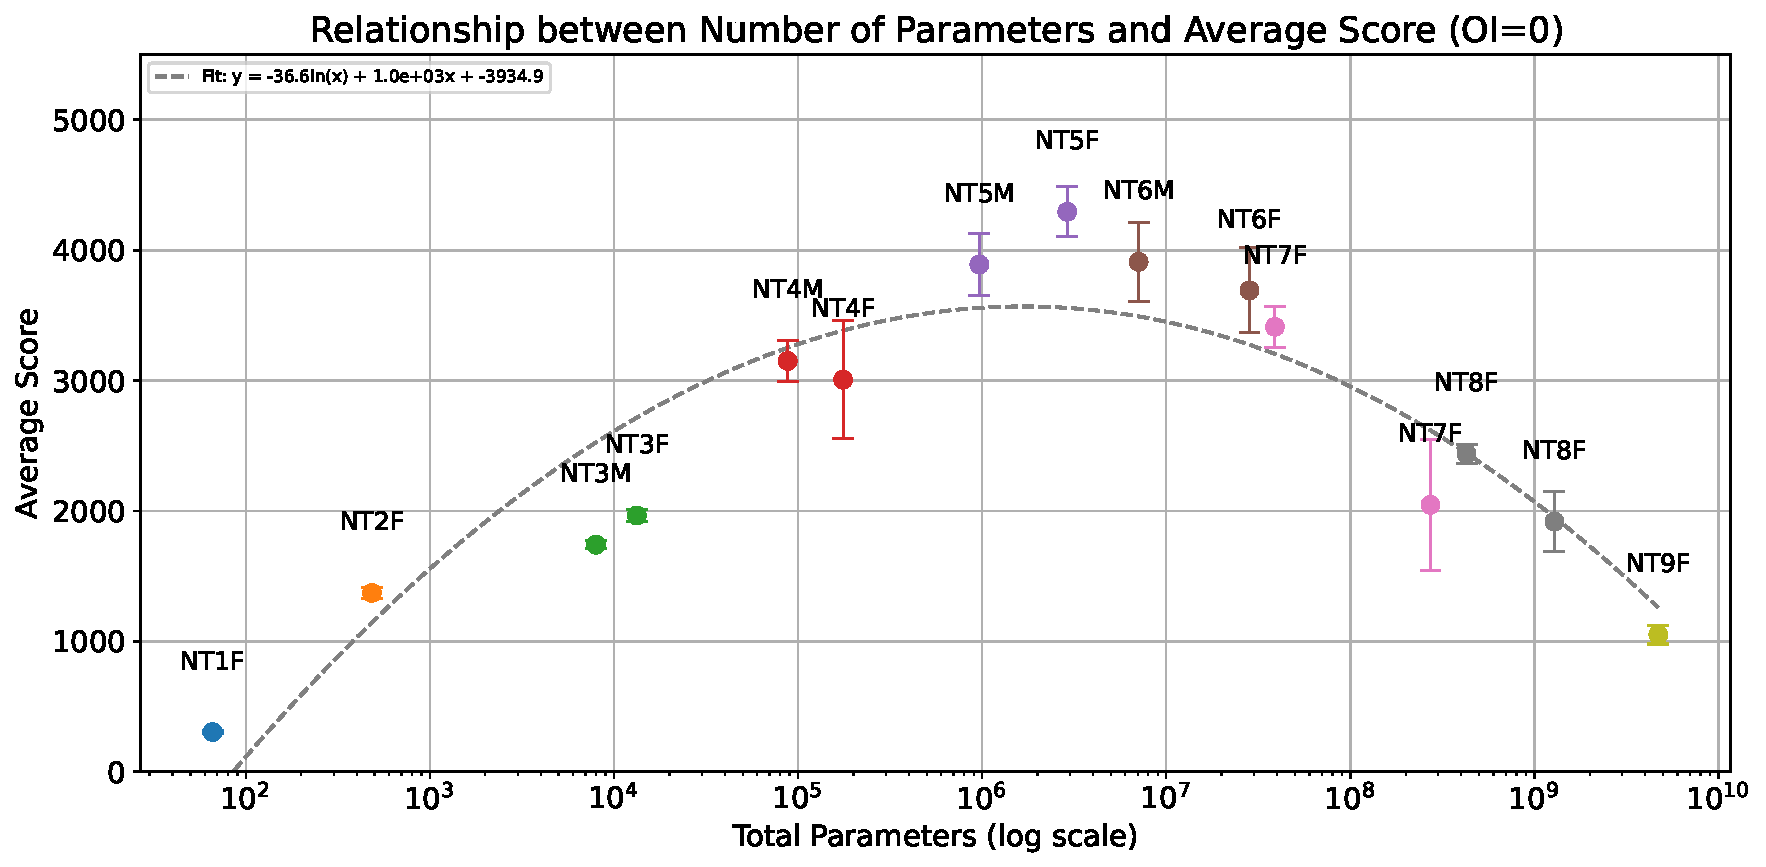
\includegraphics[width=\linewidth]{pdf/parameter_performance_plots/params_performance_OI0_EXP1.pdf}
        \caption{OI=0}
        \label{fig:score_vs_tuple_OI0}
    \end{subfigure}

    \vspace{1em}
    \begin{subfigure}[b]{\linewidth}
        \centering
        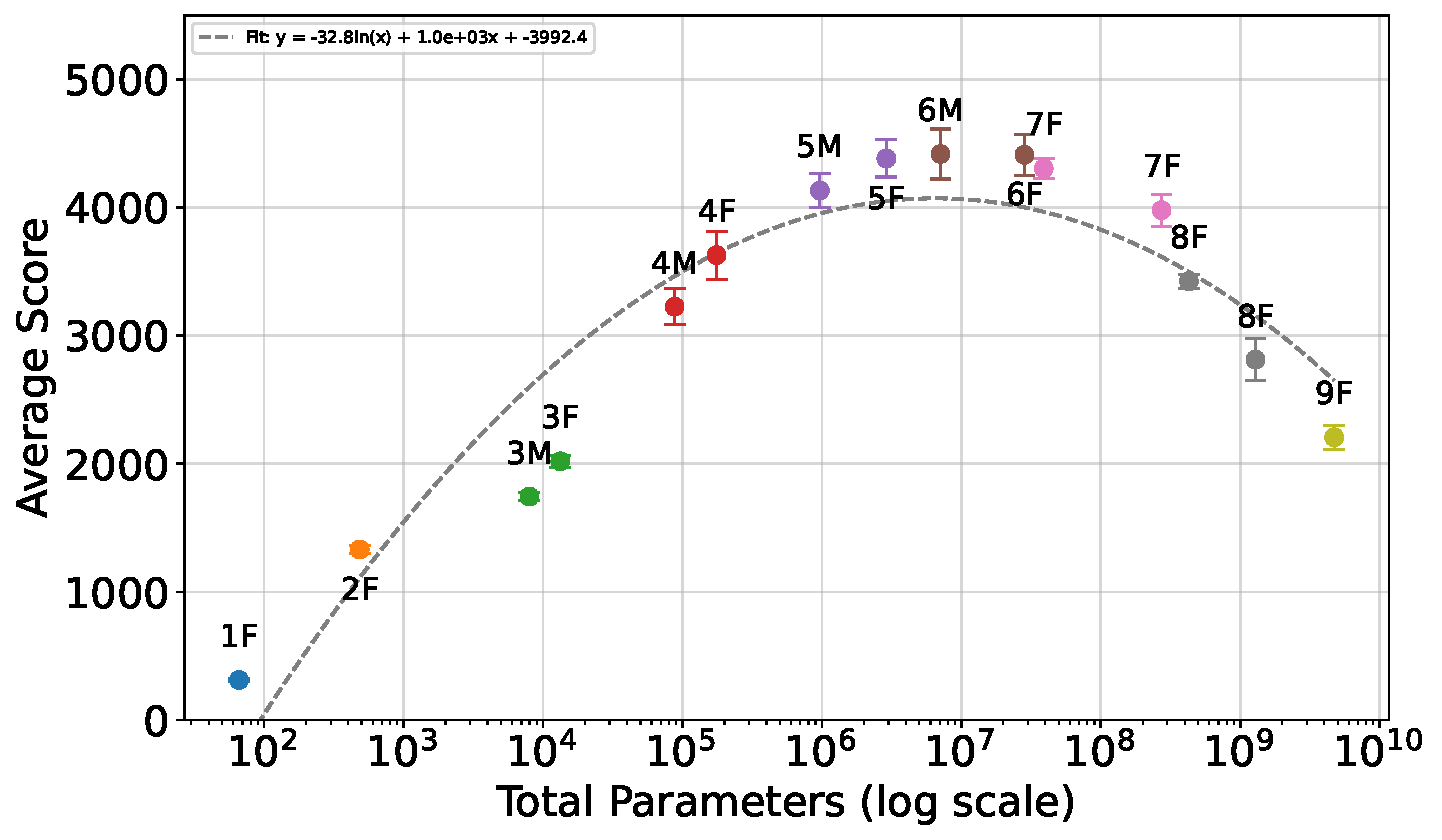
\includegraphics[width=\linewidth]{pdf/parameter_performance_plots/params_performance_OI1200_EXP1.pdf}
        \caption{OI=1200}
        \label{fig:score_vs_tuple_OI1200}
    \end{subfigure}

    \vspace{1em}
    \begin{subfigure}[b]{\linewidth}
        \centering
        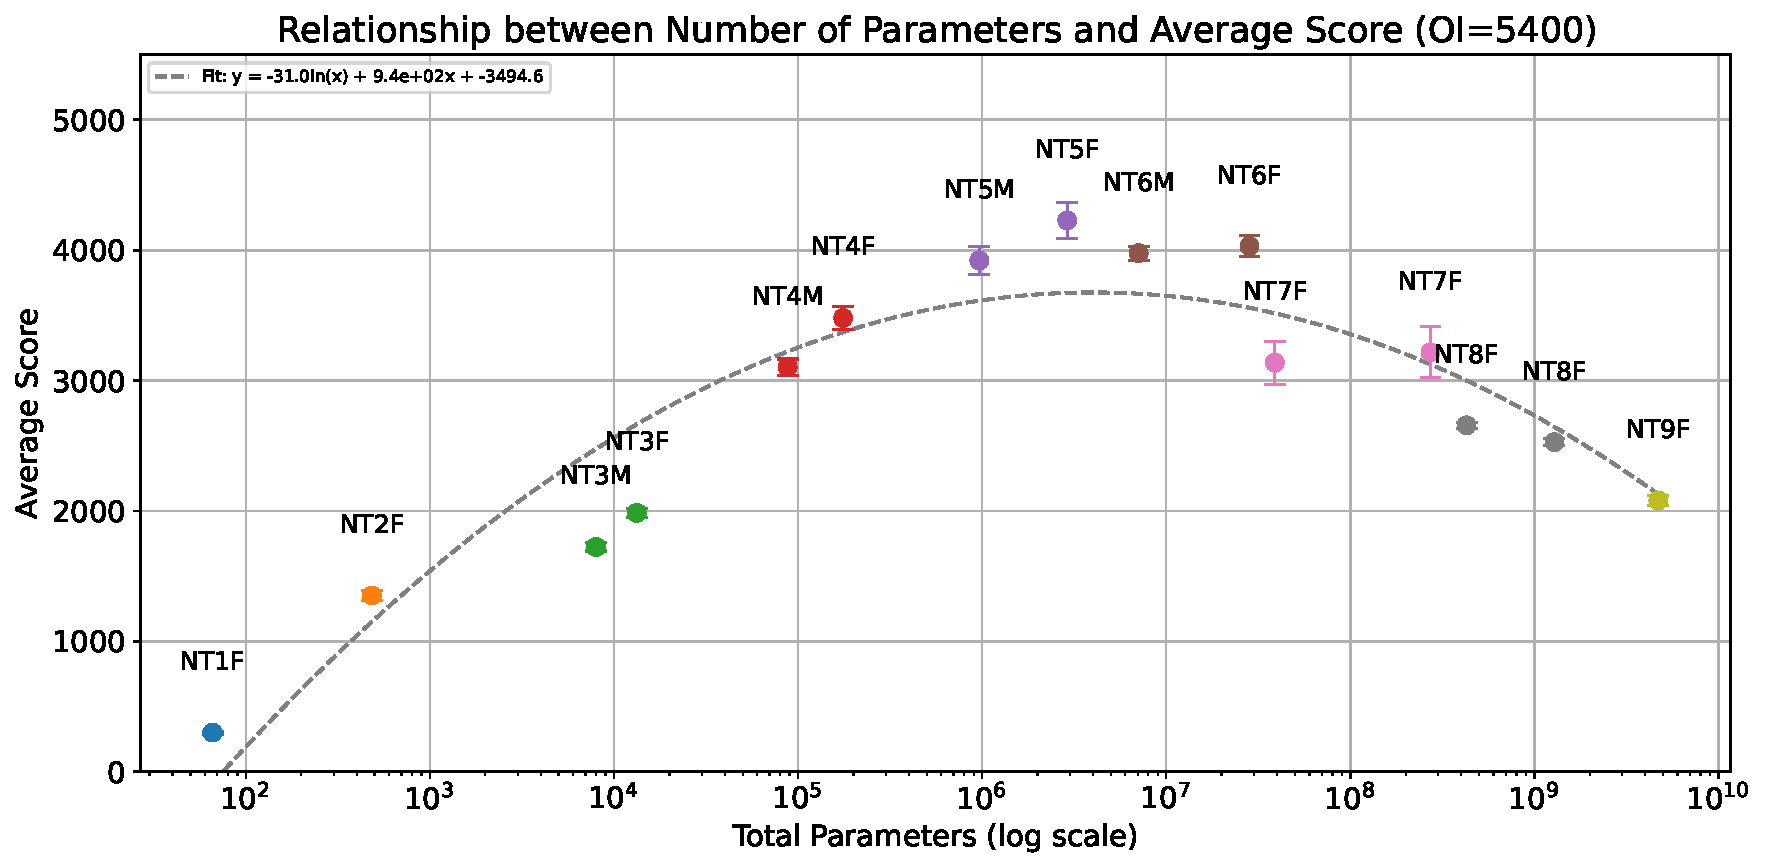
\includegraphics[width=\linewidth]{pdf/parameter_performance_plots/params_performance_OI5400_EXP1.pdf}
        \caption{OI=5400}
        \label{fig:score_vs_tuple_OI5400}
    \end{subfigure}

    \caption{Greedyプレイにおいて,パラメータ数と平均スコアの関係}
    \label{fig:score_vs_tuple_all}
\end{figure}

\begin{figure}[t]
    \centering
    \begin{subfigure}[b]{\linewidth}
        \centering
        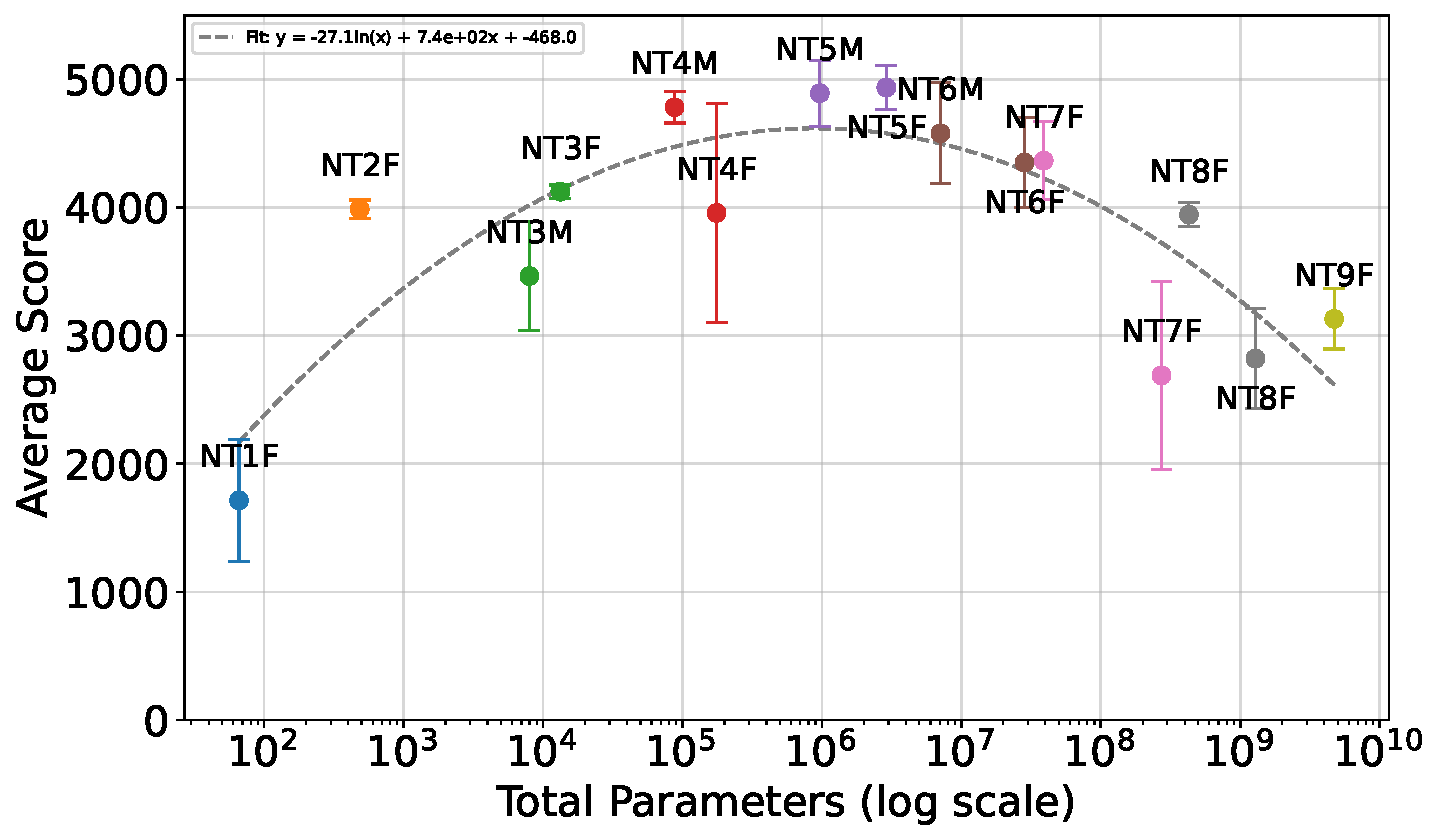
\includegraphics[width=\linewidth]{pdf/parameter_performance_plots/params_performance_OI0_EXP6.pdf}
        \caption{OI=0}
        \label{fig:score_vs_tuple_OI0_EXP6}
    \end{subfigure}

    \vspace{1em}
    \begin{subfigure}[b]{\linewidth}
        \centering
        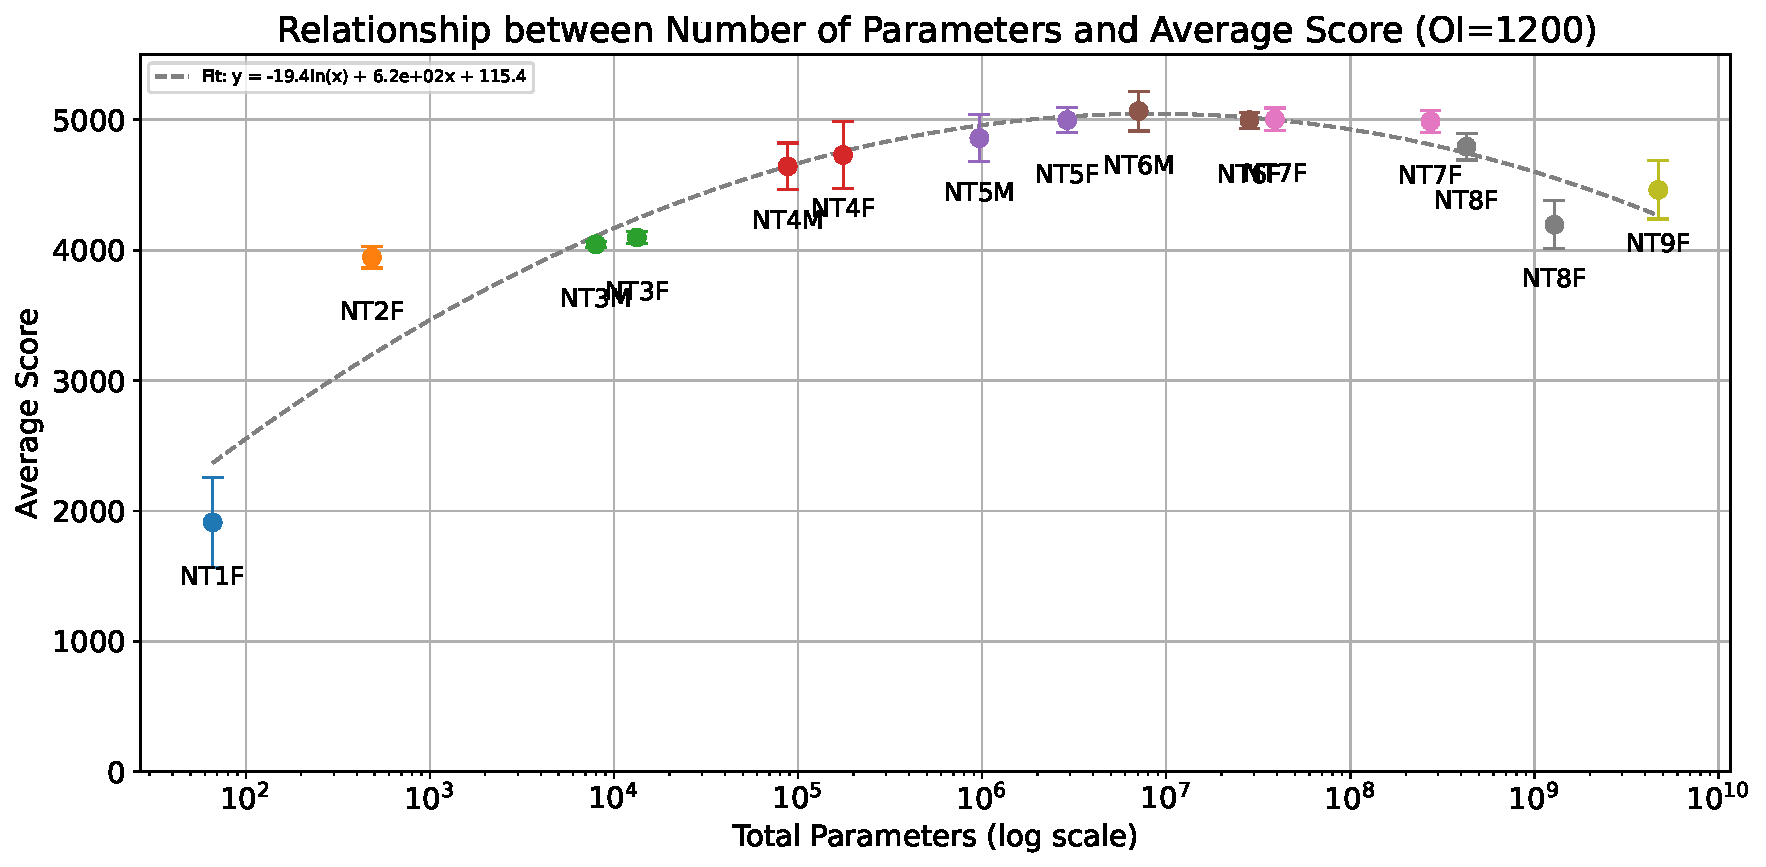
\includegraphics[width=\linewidth]{pdf/parameter_performance_plots/params_performance_OI1200_EXP6.pdf}
        \caption{OI=1200}
        \label{fig:score_vs_tuple_OI1200_EXP6}
    \end{subfigure}

    \vspace{1em}
    \begin{subfigure}[b]{\linewidth}
        \centering
        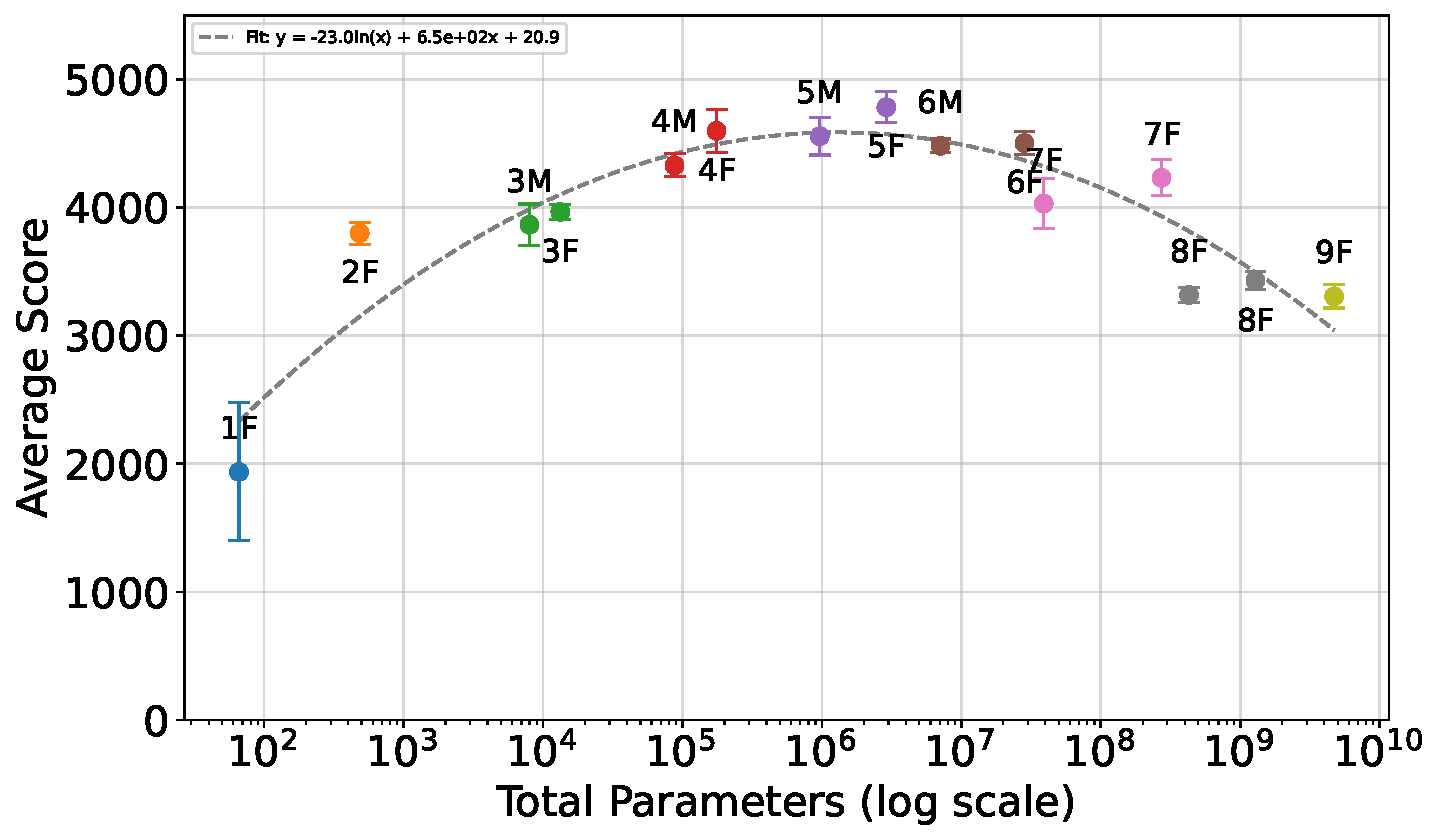
\includegraphics[width=\linewidth]{pdf/parameter_performance_plots/params_performance_OI5400_EXP6.pdf}
        \caption{OI=5400}
        \label{fig:score_vs_tuple_OI5400_EXP6}
    \end{subfigure}

    \caption{Expectimax深さ6において,パラメータ数と平均スコアの関係}
    \label{fig:score_vs_tuple_all_EXP6}
\end{figure}

次に,RQ1 と RQ3 について考察するため,深さ6のExpectimax探索を行った場合の,Nタプルネットワークのパラメータ数と平均スコアを関係を図\ref{fig:score_vs_tuple_OI0_EXP6}から図\ref{fig:score_vs_tuple_OI5400_EXP6}に示す.
各グラフの近似曲線から,いずれのグラフもおよそ放物線を描いていること,いずれの平均スコアもGreedyプレイのスコアよりも高いことが確認できた.

$\mathit{OI}=0$ の場合,探索を行ってもスコアのばらつきはそれほど小さくならず,特に Full のものについてばらつきが大きい傾向が見られる.
これはパラメータ数が多い方が評価値の修正が起こり難く,局所最適解から抜け出しにくいのではないかと考えられる.

$\mathit{OI}=1200$ の場合,\textsf{5M}から\textsf{7F}まで同程度の平均スコアを達成しており,放物線の上昇と下降の傾きが小さい.
これは,強いプレイヤが達成しうるスコアの上限に近づいていて向上の余地が小さいことと,弱いプレイヤが探索によってスコアを上昇させられることを示唆する.
$\mathit{OI}=5400$ の場合には,スコアのばらつきは小さいものの,放物線の形やスコアの最大は $\mathit{OI}=0$ の場合のそれらとあまり変わらなかった.


\begin{figure}[t]
    \centering
    \begin{subfigure}[b]{\linewidth}
        \centering
        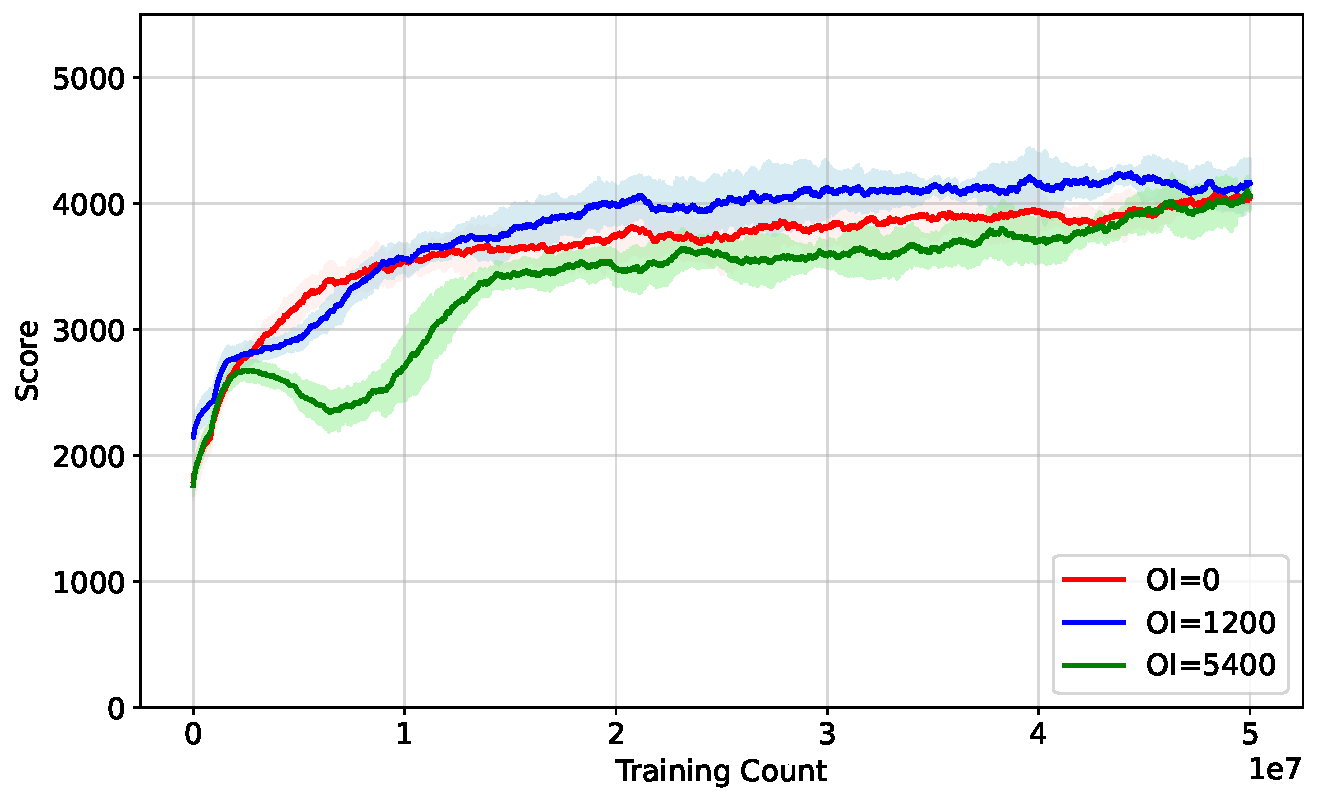
\includegraphics[width=\linewidth]{pdf/learning_progress_plots/learning_progress_NT5M_tuple298_combined.pdf}
        \caption{5Mの学習過程のスコアの変化}
        \label{fig:learning_progress_NT5M}
    \end{subfigure}

    \vspace{1em}
    \begin{subfigure}[b]{\linewidth}
        \centering
        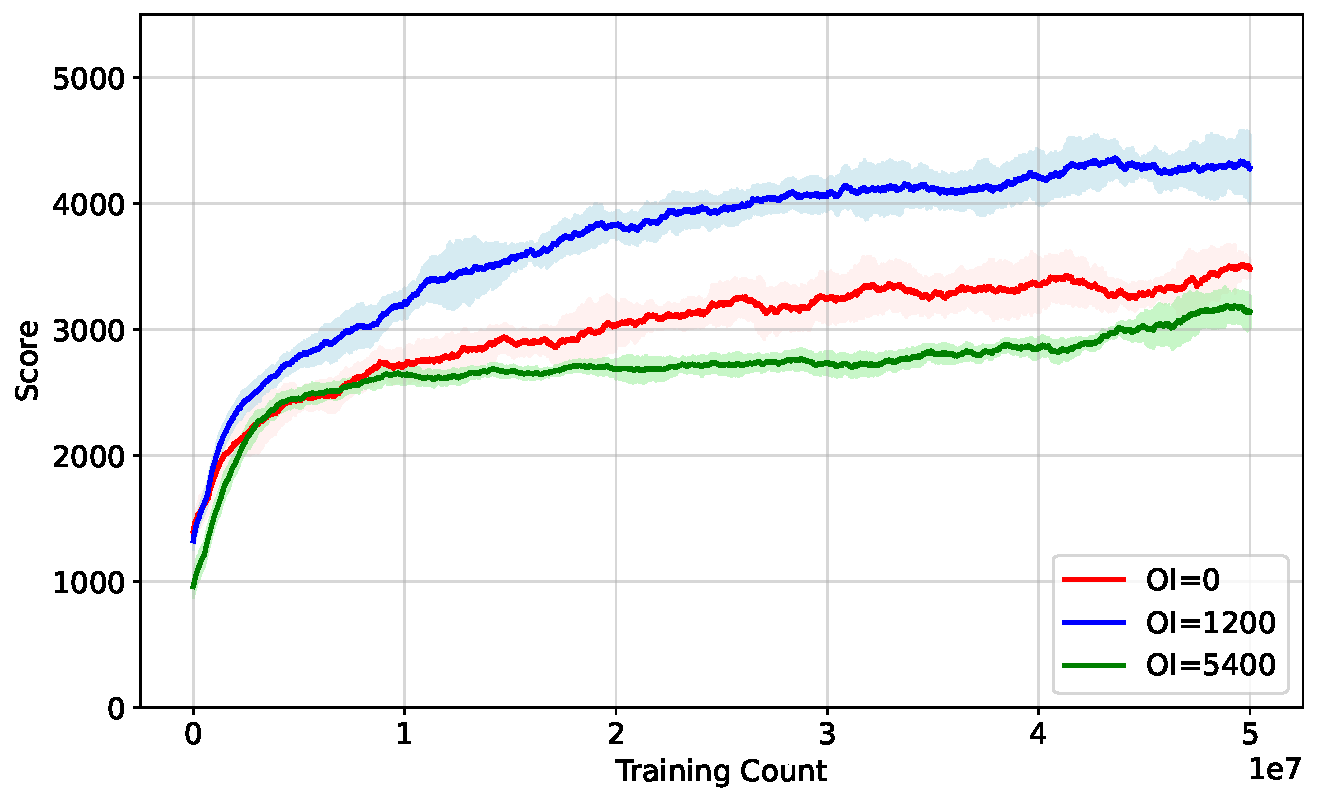
\includegraphics[width=\linewidth]{pdf/learning_progress_plots/learning_progress_NT7F_tuple0_combined.pdf}
        \caption{7Fの学習過程のスコアの変化}
        \label{fig:learning_progress_NT7F}
    \end{subfigure}

    \caption{5Mと7Fの学習推移の比較}
    \label{fig:learning_progress_comparison}
\end{figure}

\subsection{学習の進み方の比較}
図\ref{fig:learning_progress_comparison}は,5Mと7Fの学習の際のスコアの推移を示している.
このグラフではy軸にスコア,x軸に学習回数を取り,各学習回数ごとのスコアの平均を求め,
それを学習回数10000ごとに移動平均を取り,グラフにプロットしている.

OIの初期値を0に設定した場合(図\ref{fig:NT5M_OI0_learning_progress},図\ref{fig:NT7F_OI0_learning_progress}),NT5Mは学習が進むにつれてスコアが上昇しているが,NT7Fはスコアが上昇しないことが確認できた.
これは7Fが局所最適解にハマっていることを示している.
OIの初期値を1200に設定した場合(図\ref{fig:NT5M_OI1200_learning_progress},図\ref{fig:NT7F_OI1200_learning_progress}),NT5MとNT7Fの両方のスコアの上昇が緩やかになり,
5Mの場合学習途中スコアとしては約2800点ほどで一度停滞が入り,その後再び上昇に転じている.
このスコアの停滞しているのは表\ref{specific}を見ると256タイルが完成してから512タイルが完成するまでの間であることが分かる.
この停滞期の盤面は盤面に比較的空きタイルがあり,色んな手を選択することで効率の悪い手を選んでしまい停滞しているのではないかと考えている.
また,7FはOIの初期値を1200に設定した場合,序盤のスコアの上昇が緩やかになっているのも同じ原因ではないかと考える.
OIの初期値を5400に設定した場合(図\ref{fig:NT5M_OI5400_learning_progress},図\ref{fig:NT7F_OI5400_learning_progress}),5Mと7Fの両方のスコアの上昇が緩やかになり,,両方とも途中で停滞が発生している.
5Mは停滞を乗り越えて大きくスコアを上昇させているが,7Fは停滞が長引き大きなスコア上昇にまで至っていないので,
学習不足であると考えている.

\subsection{パラメータ数の増加によるプレイヤの挙動の変化}
% ここからRQ1についての考察を深めるために,
OIの初期値1200のスコアが同等でパラメータ数が違う4Fと8M,5Mと7Fのプレイヤをパーフェクトプレイヤを用いて詳細な比較を行い,
パラメータ数の増加がプレイヤの挙動にどのような影響を与えるのかについて詳しく調べて行く.
指標としては,正確度,絶対誤差,生存率を用いる.
\begin{itemize}
    \item 正確度:パーフェクトプレイヤの選択した手とプレイヤの選択した手の一致率
    \item 絶対誤差:パーフェクトプレイヤの選択した手とプレイヤの選択した手のパーフェクトプレイヤ評価値の差
    \item 生存率:あるprogressにおいて,プレイヤが生存している確率
\end{itemize}

\begin{figure}[t]
\centering
\begin{subfigure}[b]{0.8\linewidth}
    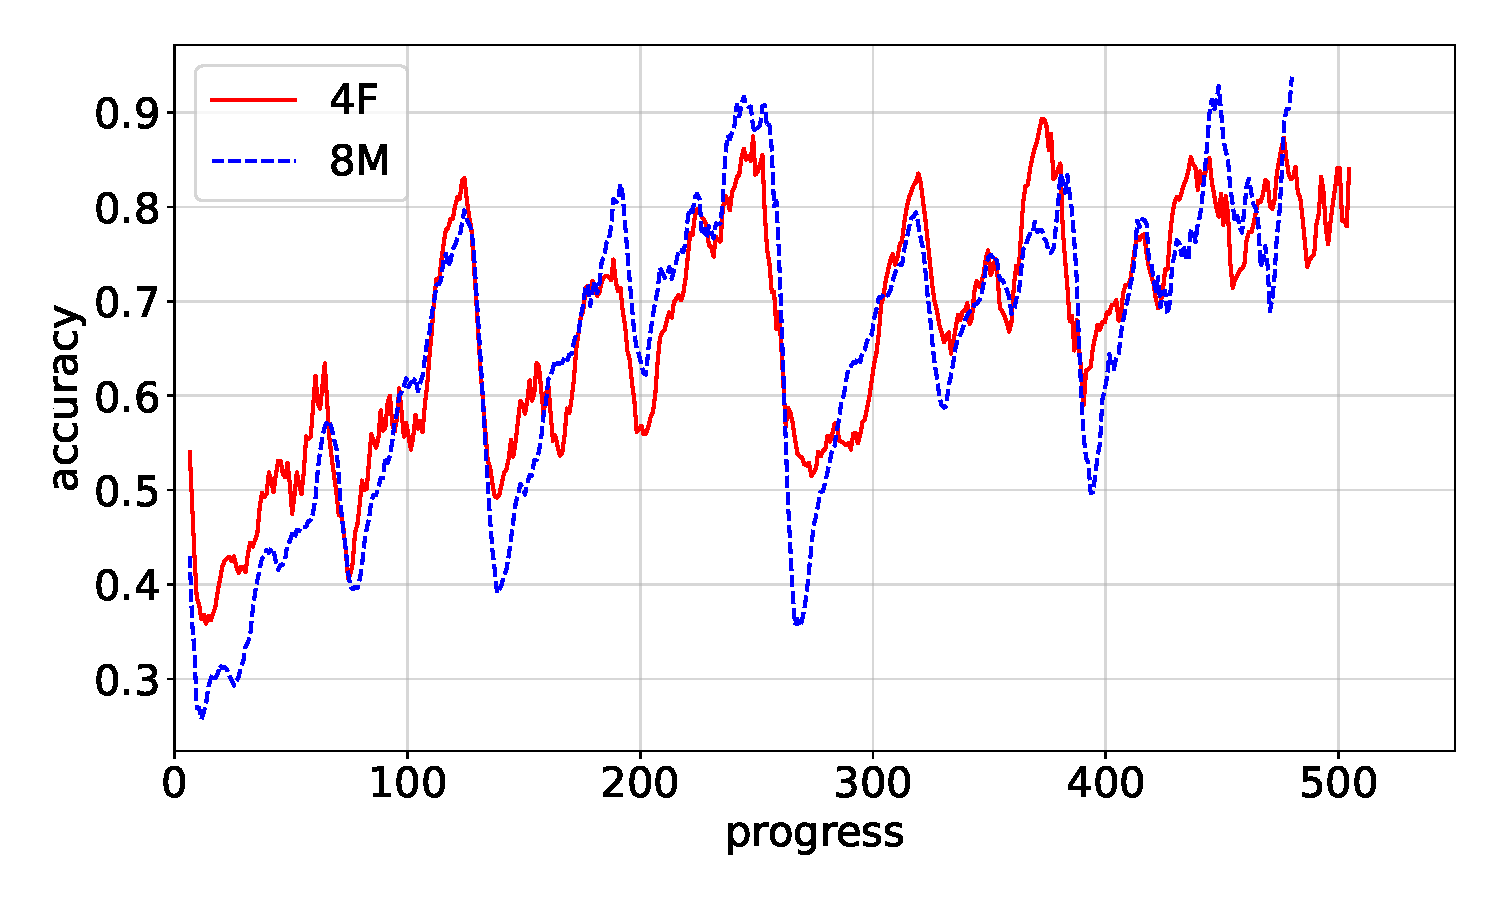
\includegraphics[width=\linewidth]{pdf/compare/NT4F_and_NT8M/accuracy.pdf}
    \caption{正確度}
    \label{fig:NT4F_and_NT8M_accuracy}
\end{subfigure}
\begin{subfigure}[b]{0.8\linewidth}
    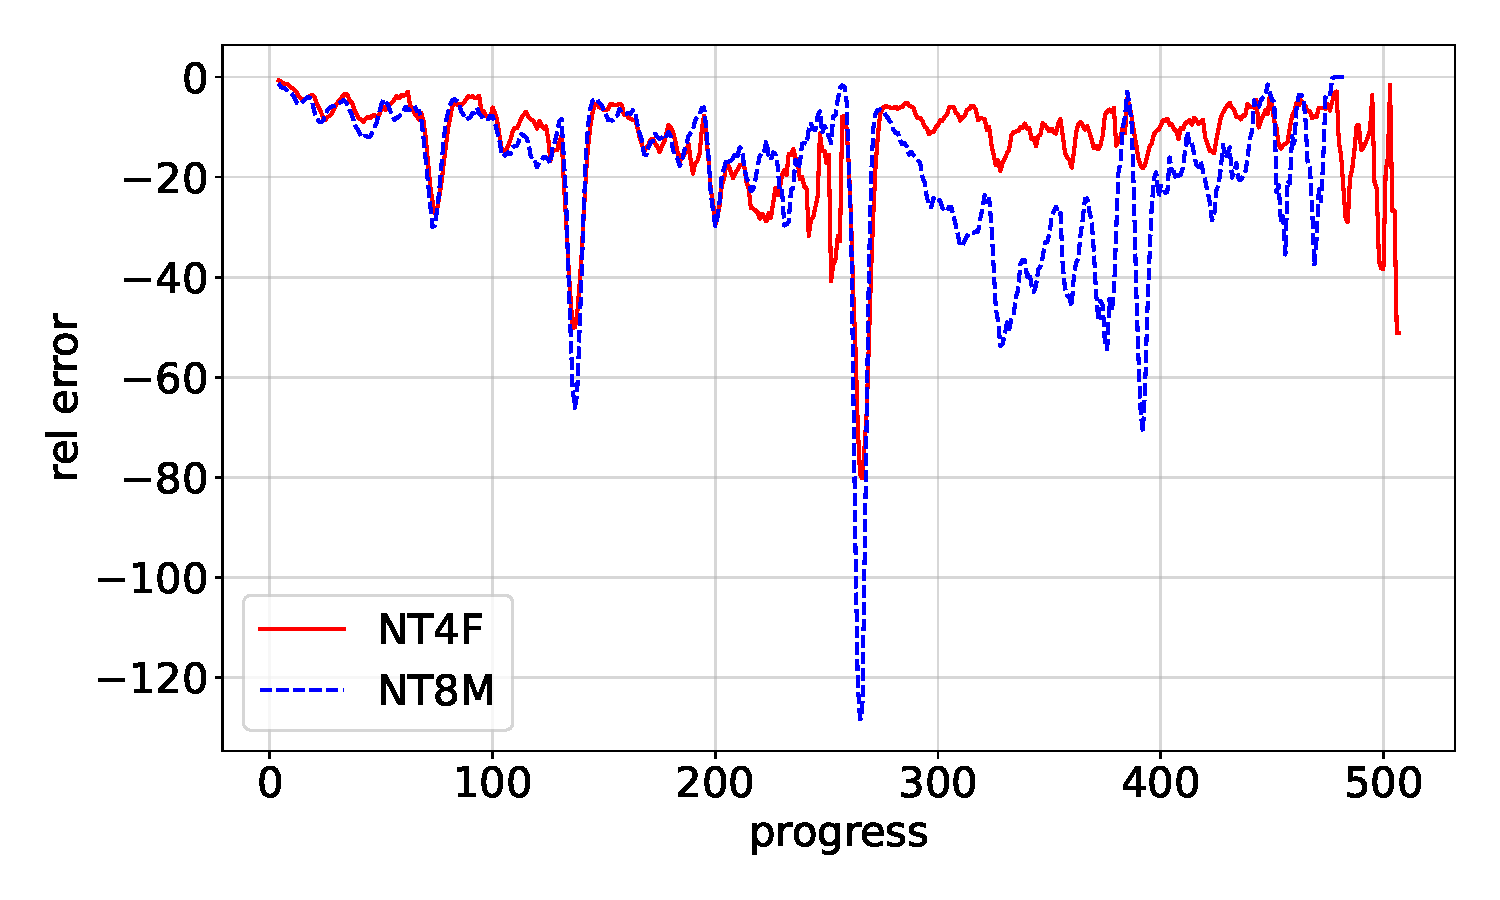
\includegraphics[width=\linewidth]{pdf/compare/NT4F_and_NT8M/error_abs.pdf}
    \caption{絶対誤差}
    \label{fig:NT4F_and_NT8M_error_abs}
\end{subfigure}
\begin{subfigure}[b]{0.8\linewidth}
    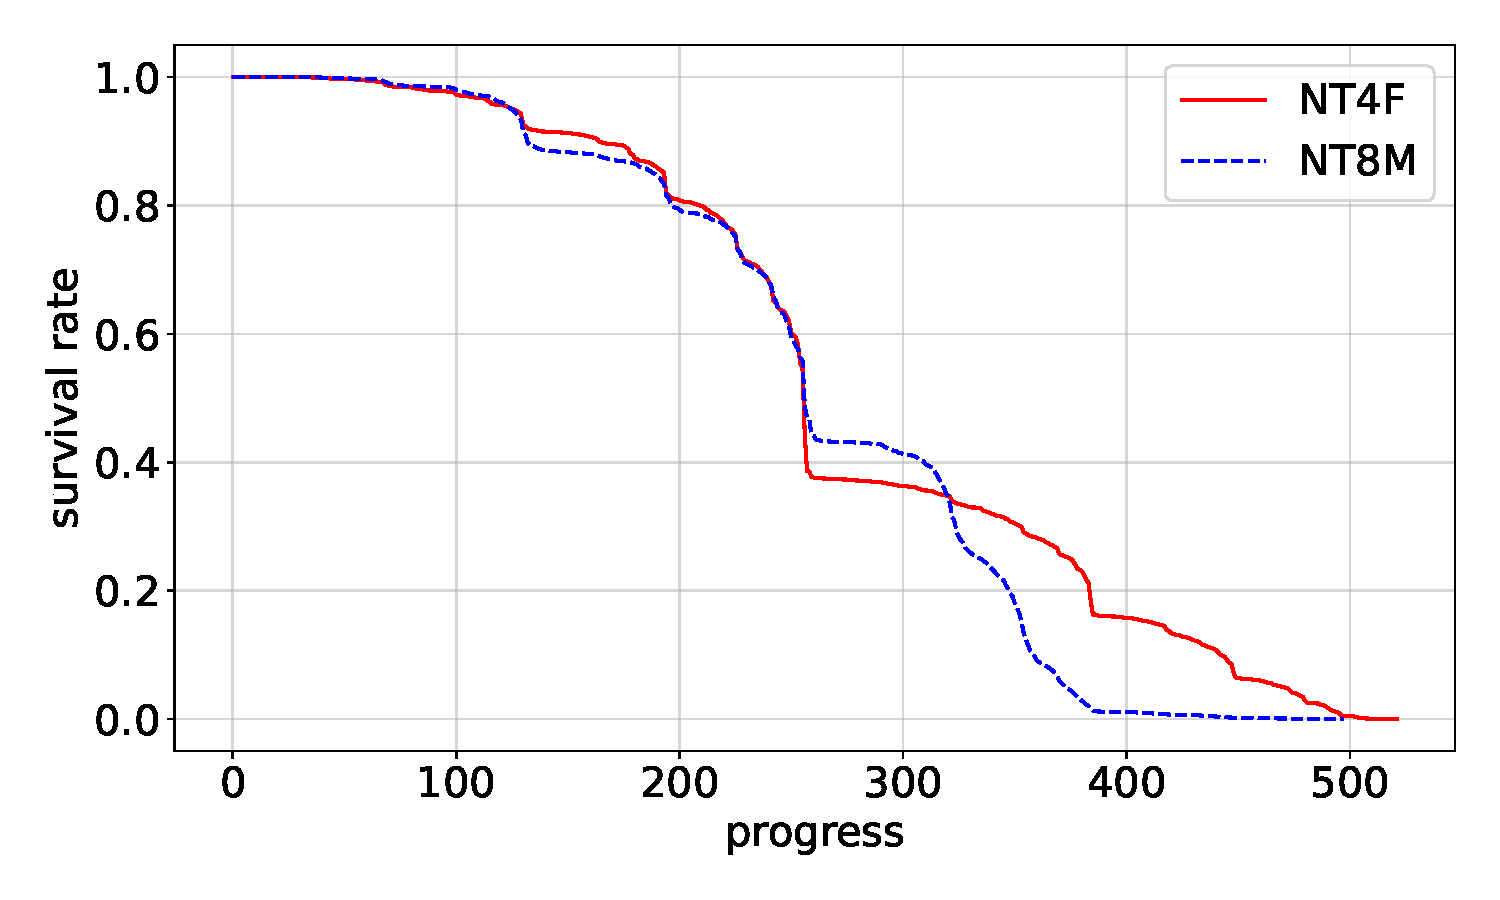
\includegraphics[width=\linewidth]{pdf/compare/NT4F_and_NT8M/survival.pdf}
    \caption{生存率}
    \label{fig:NT4F_and_NT8M_survival}
\end{subfigure}
\caption{4Fと8Mの比較結果}
\label{fig:NT4F_and_NT8M_results}
\end{figure}

まず初めに図\ref{fig:NT4F_and_NT8M_results}は,4Fと8MのプレイヤのGreedyプレイの比較を示している.
図\ref{fig:NT4F_and_NT8M_accuracy}は,を見ると正確度のグラフはどちらも同じような形をしているが,8Mの方が上下に大きく変動していることが分かる.
図\ref{fig:NT4F_and_NT8M_error_abs_diff}を見ると4Fの方が8M多くのprogressで絶対誤差が小さいことが分かる,これはprogress260を超えた辺りから顕著に現れている.
progress260辺りは512のタイルが完成し以前と似ている盤面になるのだが,8Mタプルサイズが大きくなることで汎化性能が落ちて,
序盤の盤面と全く別物として学習してしまい,512タイルが完成した後の盤面に対して正確度が下がり,絶対誤差も大きくなってるのではないかと考えられる.
これは図\ref{fig:NT4F_and_NT8M_survival}の生存率にも表れていて生存率ではミスをした後のprogress300を超えた辺りから顕著に生存率が8Mの生存率が下がっている.

\begin{figure}[t]
\centering
\begin{subfigure}[b]{0.8\linewidth}
    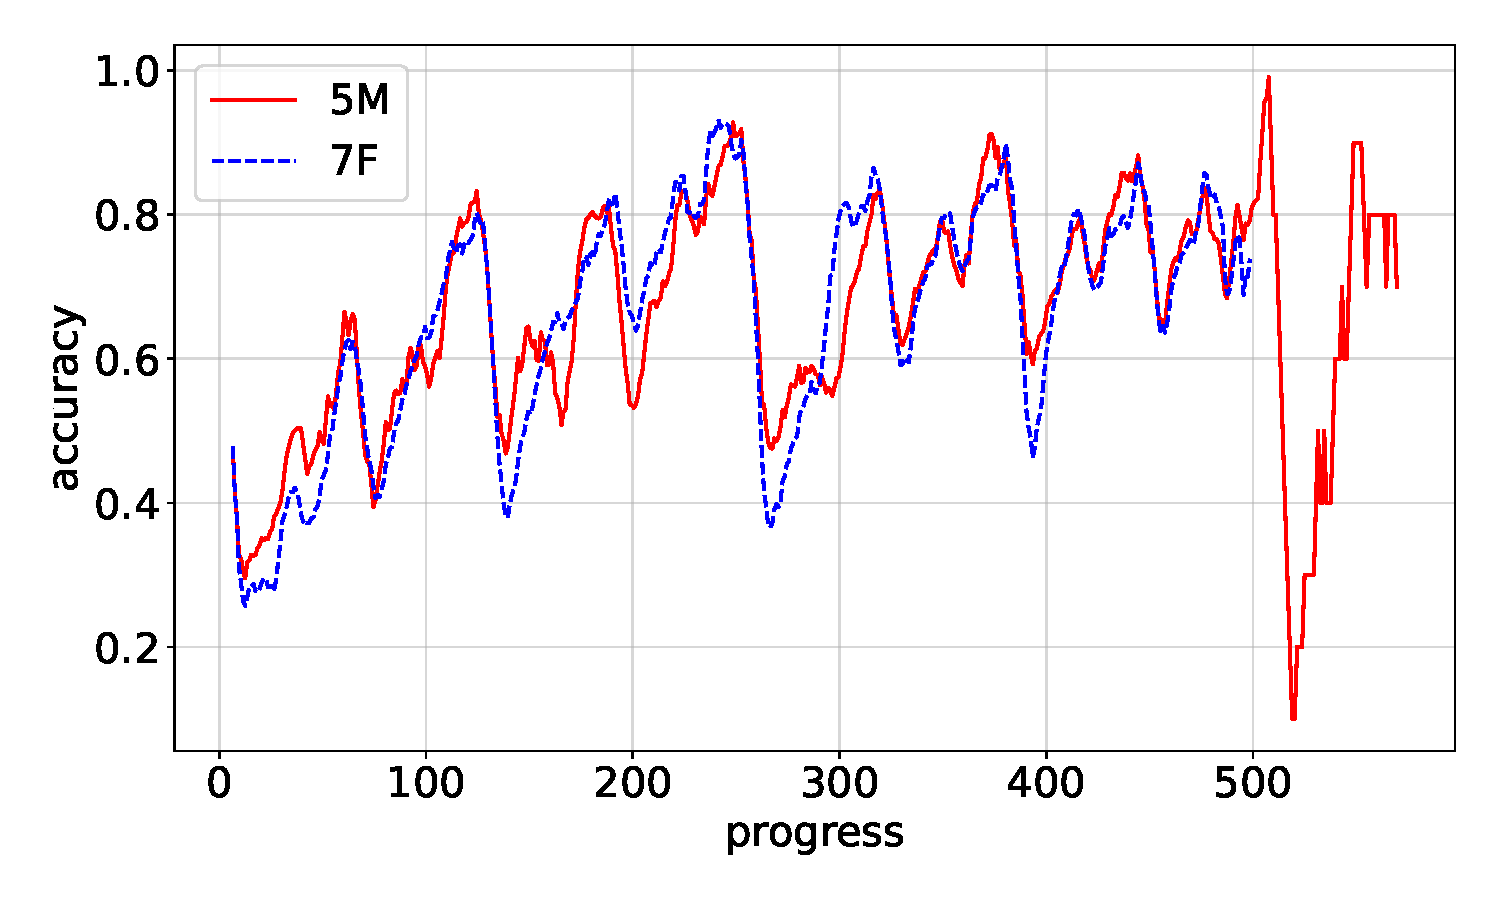
\includegraphics[width=\linewidth]{pdf/compare/NT5M_and_NT7F/accuracy.pdf}
    \caption{正確度}
    \label{fig:NT5M_and_NT7F_accuracy}
\end{subfigure}
\begin{subfigure}[b]{0.8\linewidth}
    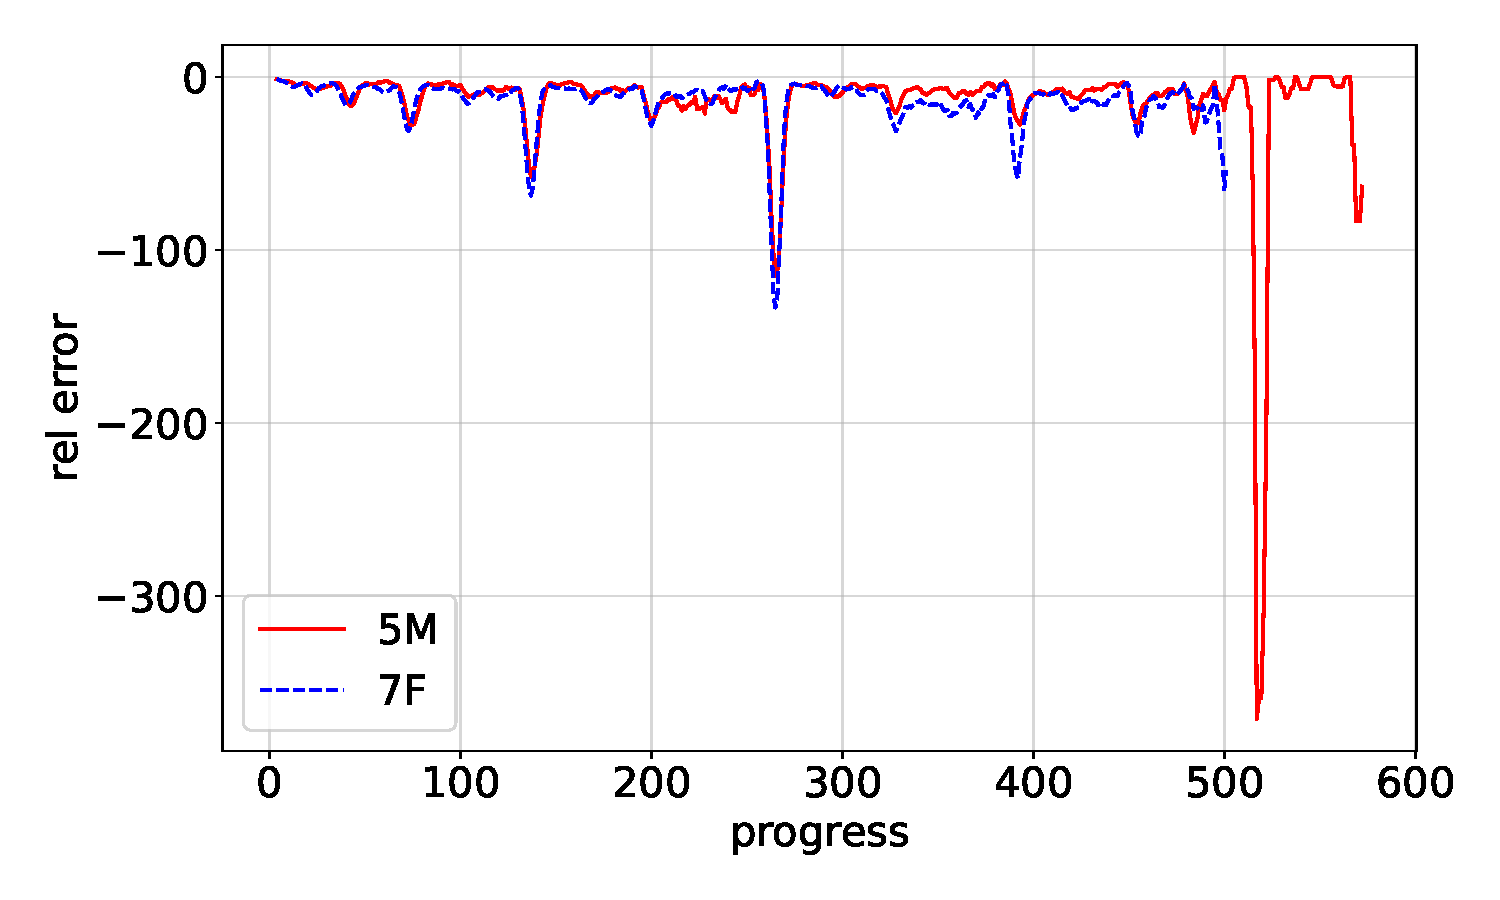
\includegraphics[width=\linewidth]{pdf/compare/NT5M_and_NT7F/error_abs.pdf}
    \caption{絶対誤差}
    \label{fig:NT5M_and_NT7F_error_abs}
\end{subfigure}
\begin{subfigure}[b]{0.8\linewidth}
    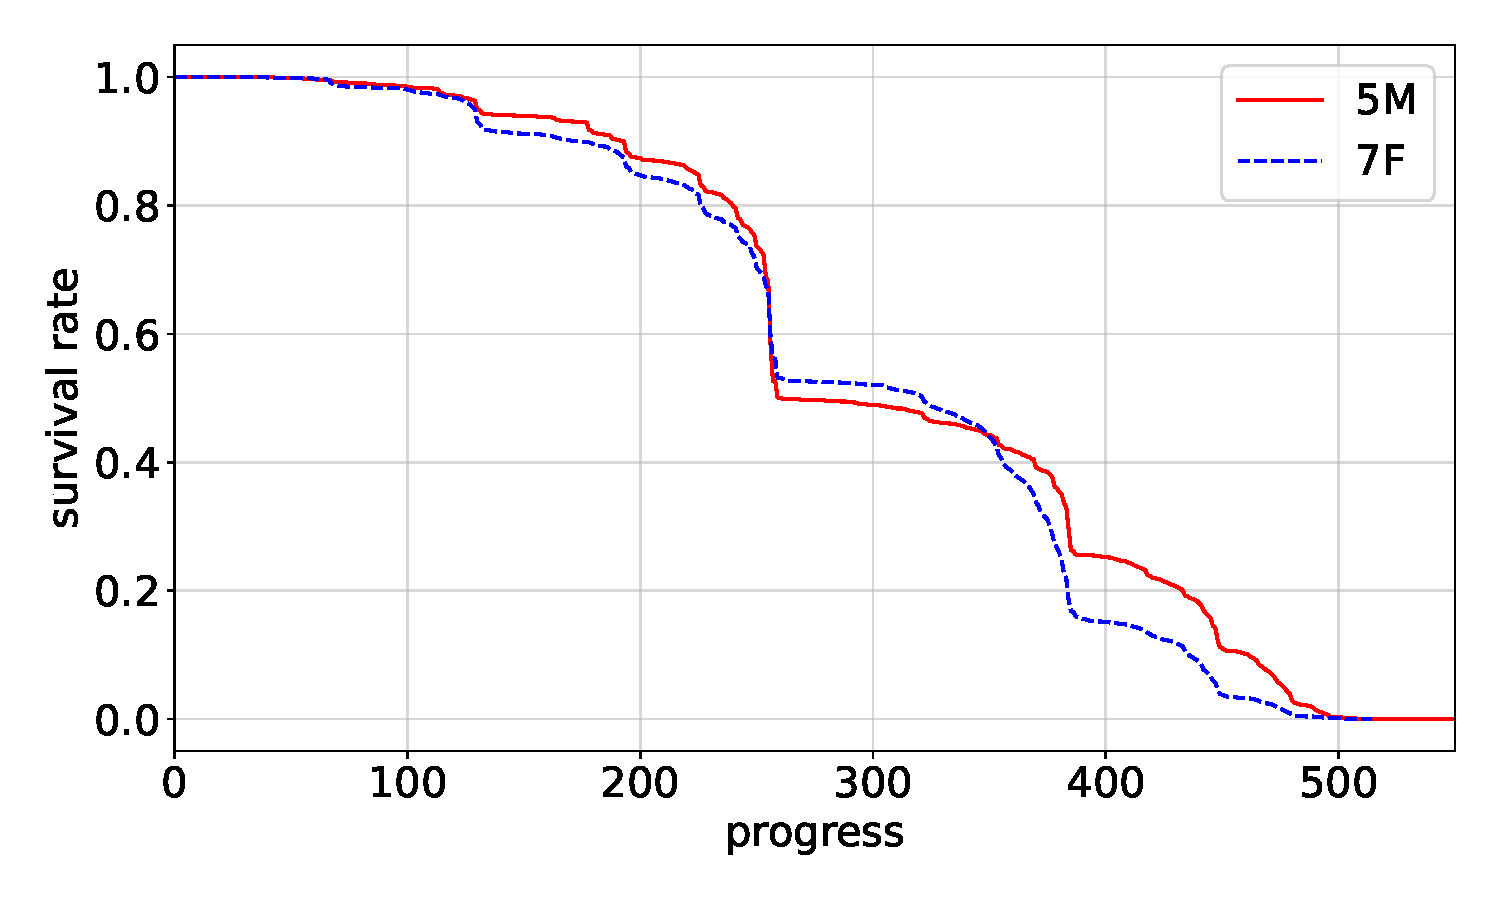
\includegraphics[width=\linewidth]{pdf/compare/NT5M_and_NT7F/survival.pdf}
    \caption{生存率}
    \label{fig:NT5M_and_NT7F_survival}
\end{subfigure}
\caption{5Mと7Fの比較結果}
\label{fig:NT5M_and_NT7F_results}
\end{figure}

次に図\ref{fig:NT5M_and_NT7F_results}は,5Mと7FのプレイヤのGreedyプレイの比較を示している.
図\ref{fig:NT5M_and_NT7F_accuracy}を見ると形は似ているが,両方の正確度が下がる場面で7Fの方が正確度が下がっているのが分かる.
図\ref{fig:NT5M_and_NT7F_error_abs}を見ると,どちらもほぼ同じ形になっていて,正確度ほど差のないグラフになっている
これは7Fは間違えても問題ない手を選んでいるだけで学習自体は十分に成功していることがわかる.
図\ref{fig:NT5M_and_NT7F_survival}を見るとどちらも上下を入れ替わりながら似たような形になっていることが分かる.
    
\begin{figure}[t]
\centering
\begin{subfigure}[b]{0.8\linewidth}
    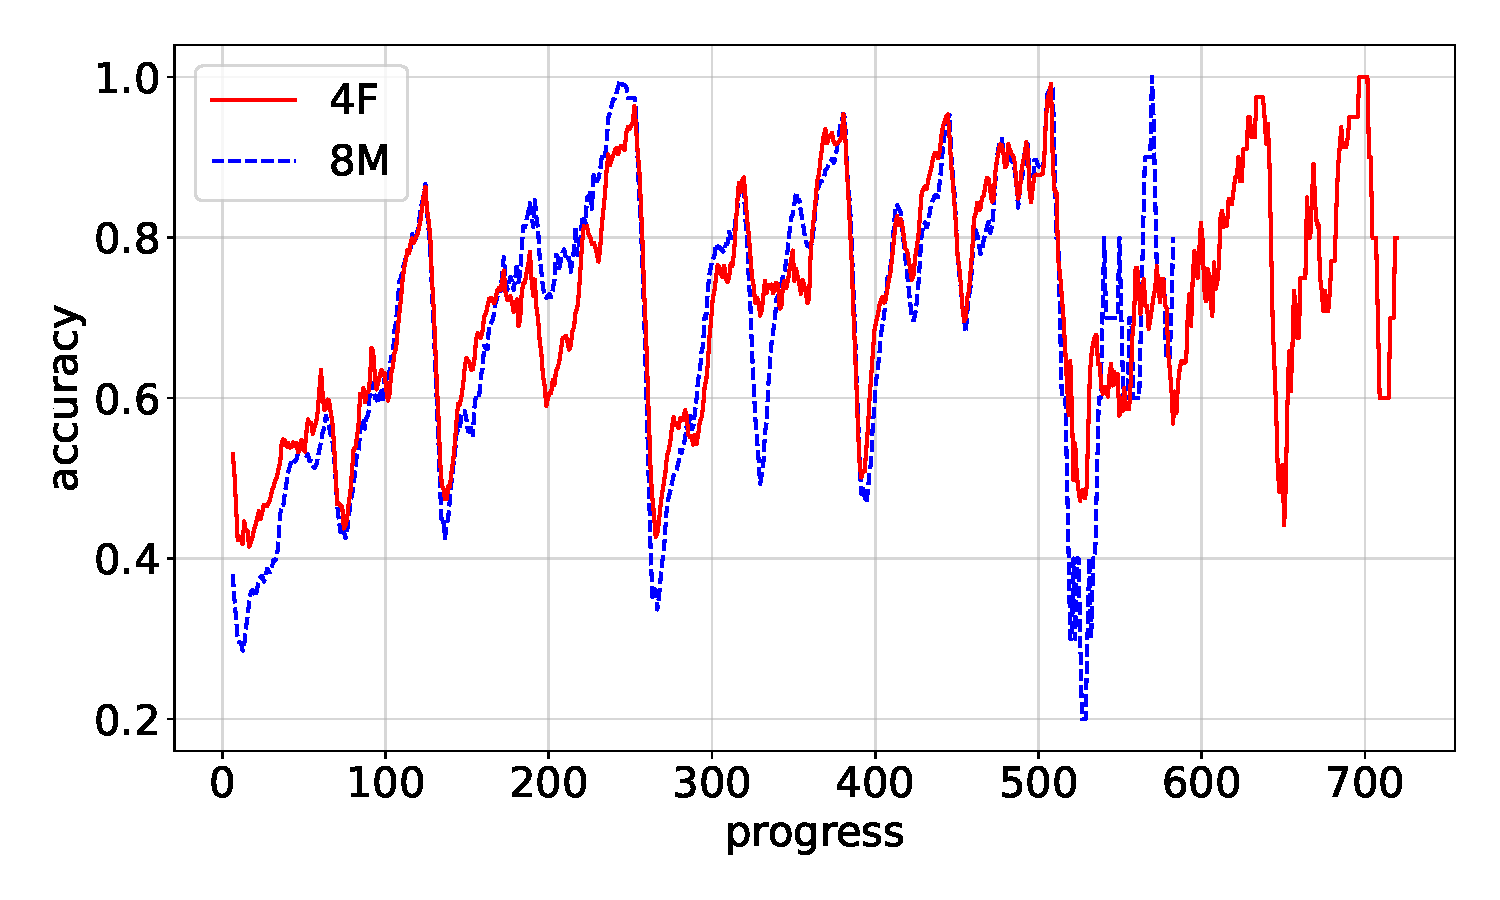
\includegraphics[width=\linewidth]{pdf/compare/EXP6_NT4F_and_NT8M/accuracy.pdf}
    \caption{正確度}
    \label{fig:EXP6_NT4F_and_NT8M_accuracy}
\end{subfigure}
\begin{subfigure}[b]{0.8\linewidth}
    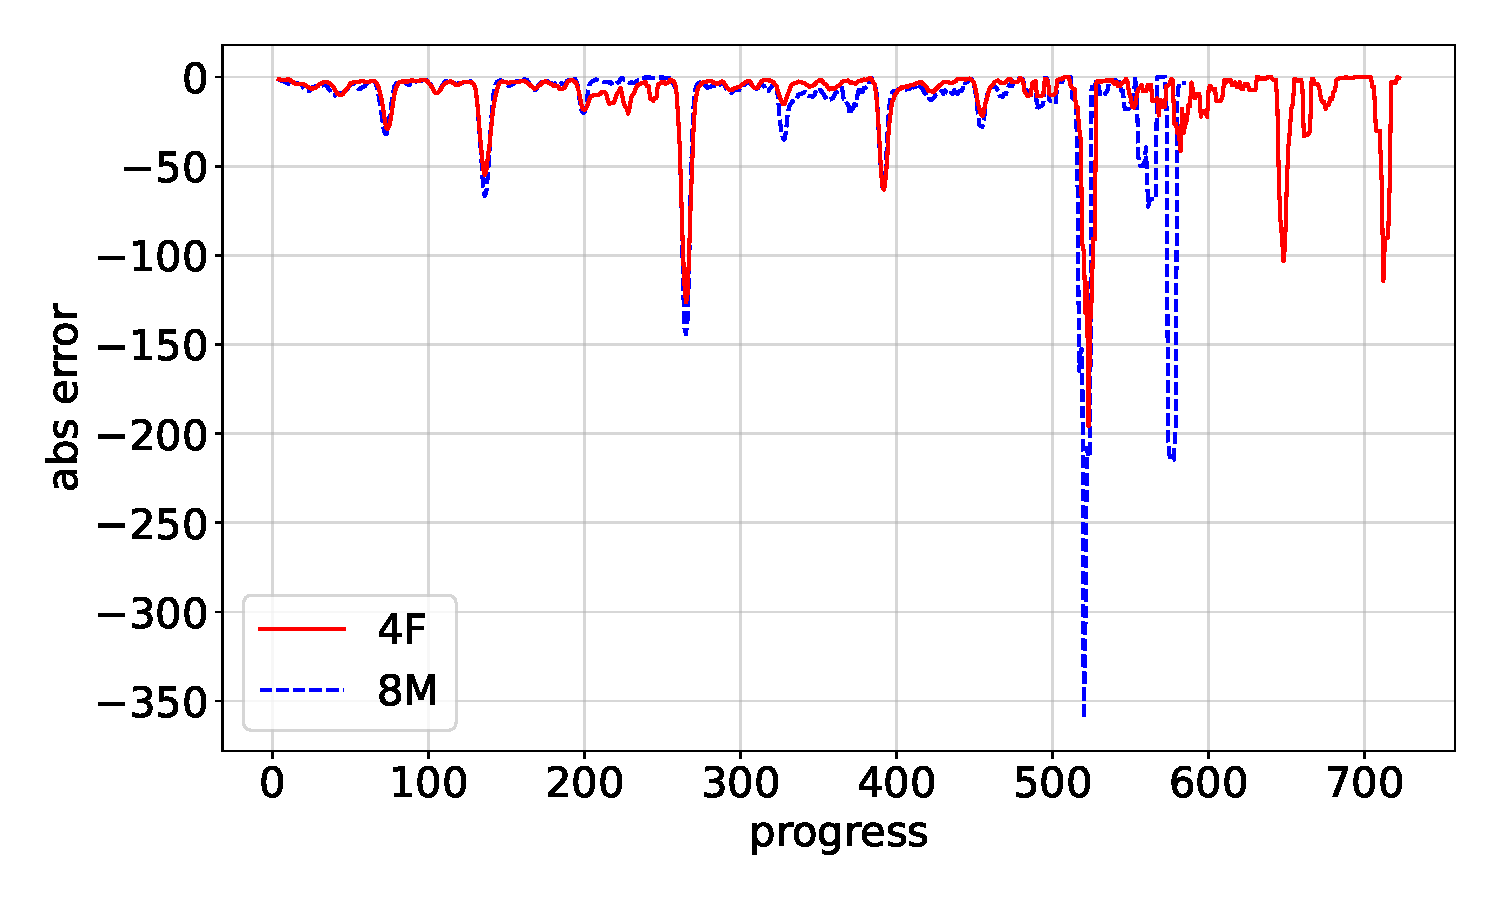
\includegraphics[width=\linewidth]{pdf/compare/EXP6_NT4F_and_NT8M/error_abs.pdf}
    \caption{絶対誤差}
    \label{fig:EXP6_NT4F_and_NT8M_error_abs}
\end{subfigure}
\begin{subfigure}[b]{0.8\linewidth}
    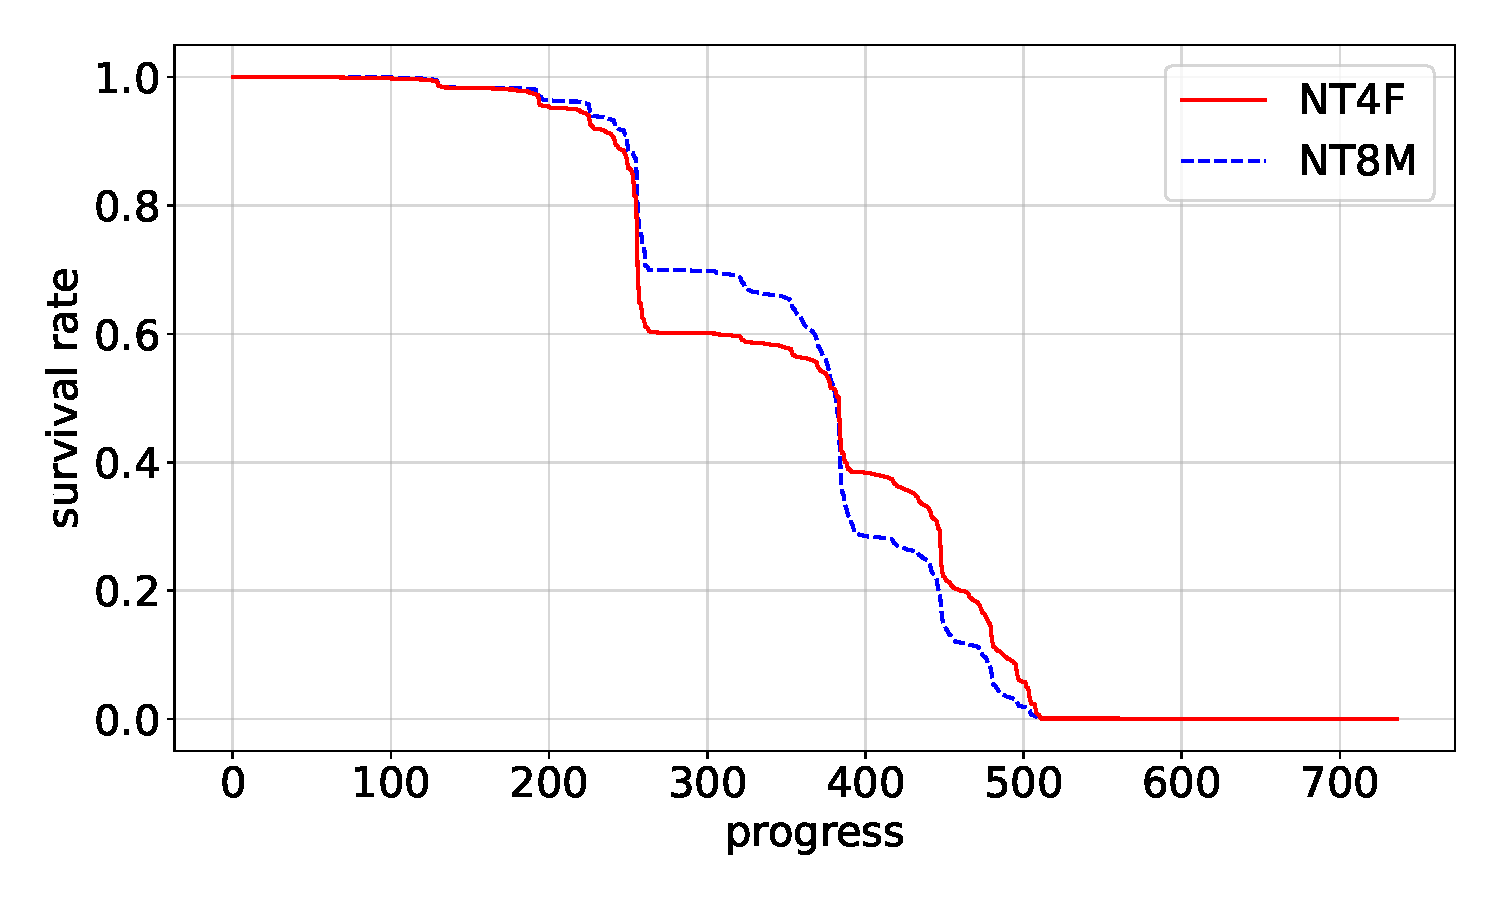
\includegraphics[width=\linewidth]{pdf/compare/EXP6_NT4F_and_NT8M/survival.pdf}
    \caption{生存率}
    \label{fig:EXP6_NT4F_and_NT8M_survival}
\end{subfigure}
\caption{4Fと8Mの比較結果(深さ6)}
\label{fig:EXP6_NT4FとNT8M_results}
\end{figure}
    

\begin{figure}[t]
\centering
\begin{subfigure}[b]{0.8\linewidth}
    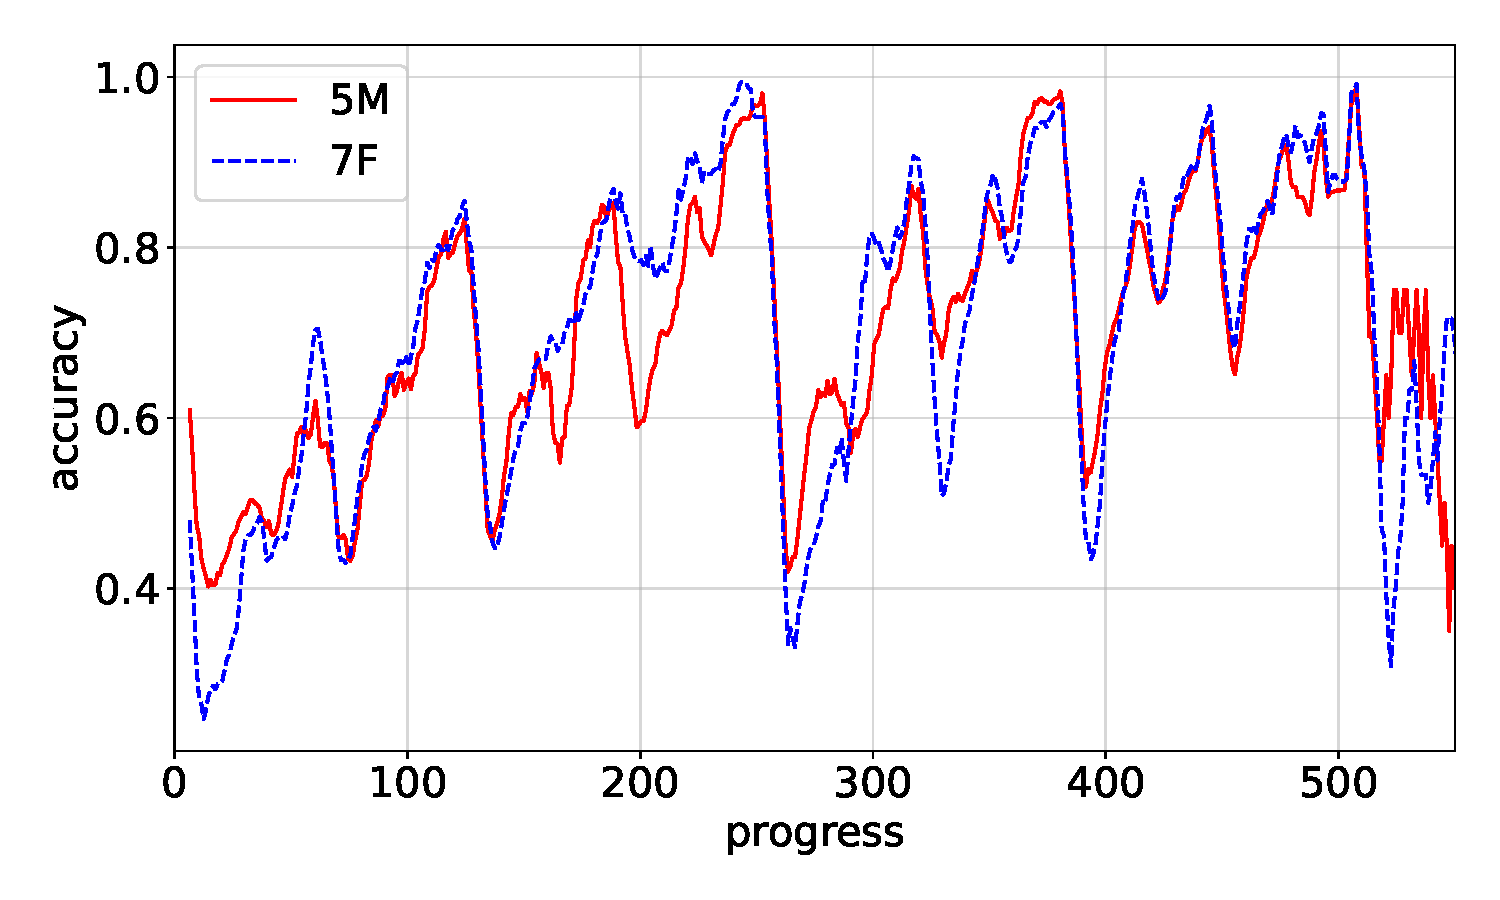
\includegraphics[width=\linewidth]{pdf/compare/EXP6_NT5M_and_NT7F/accuracy.pdf}
    \caption{正確度}
    \label{fig:EXP6_NT5M_and_NT7F_accuracy}
\end{subfigure}
\begin{subfigure}[b]{0.8\linewidth}
    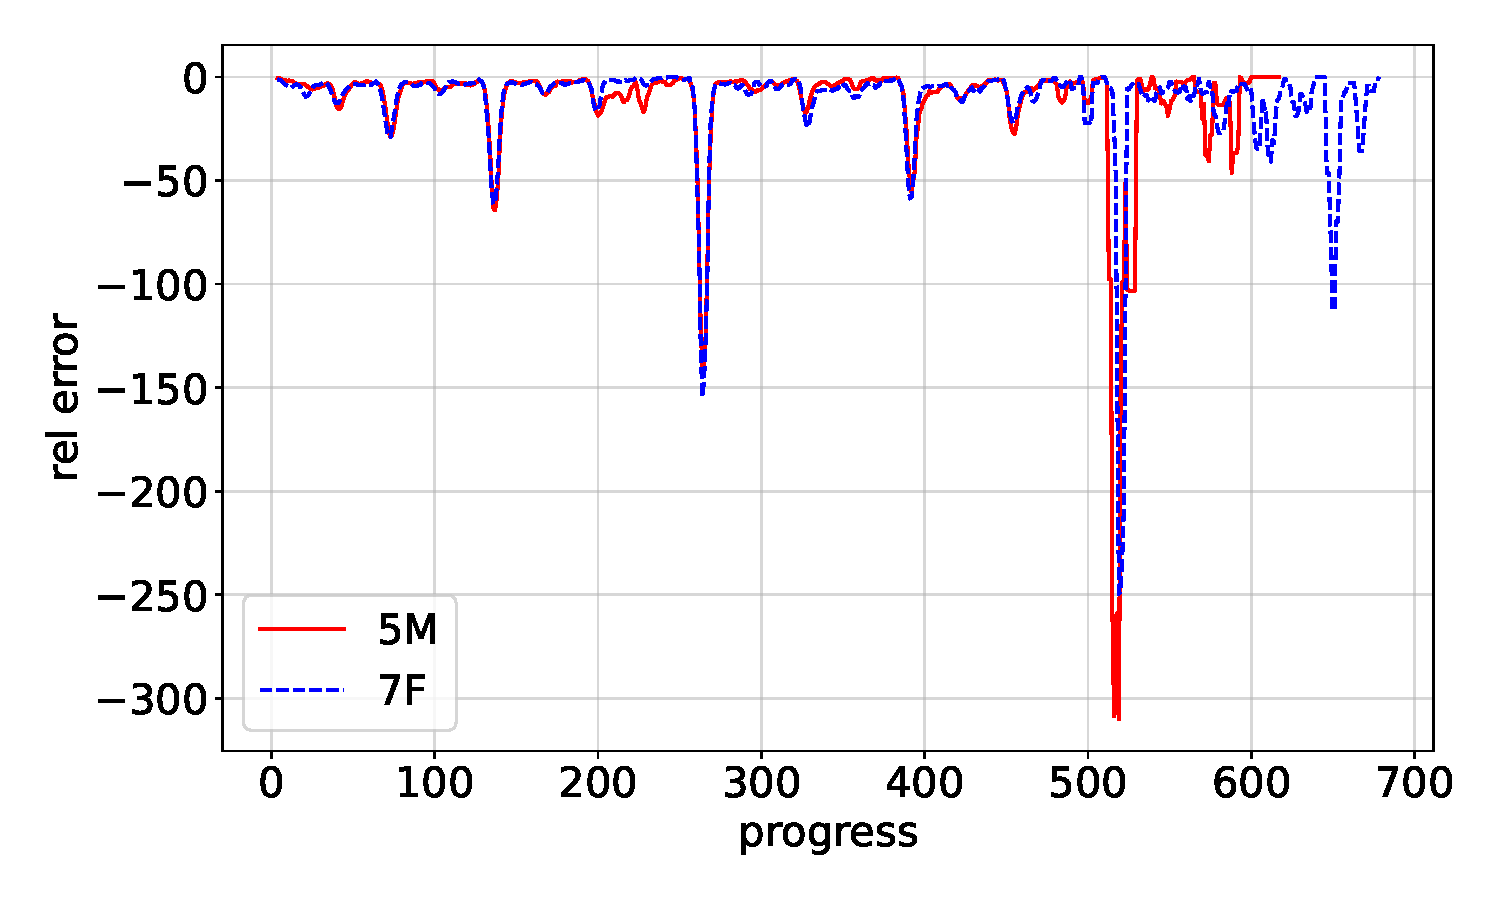
\includegraphics[width=\linewidth]{pdf/compare/EXP6_NT5M_and_NT7F/error_abs.pdf}
    \caption{絶対誤差}
    \label{fig:EXP6_NT5M_and_NT7F_error_abs}
\end{subfigure}
\begin{subfigure}[b]{0.8\linewidth}
    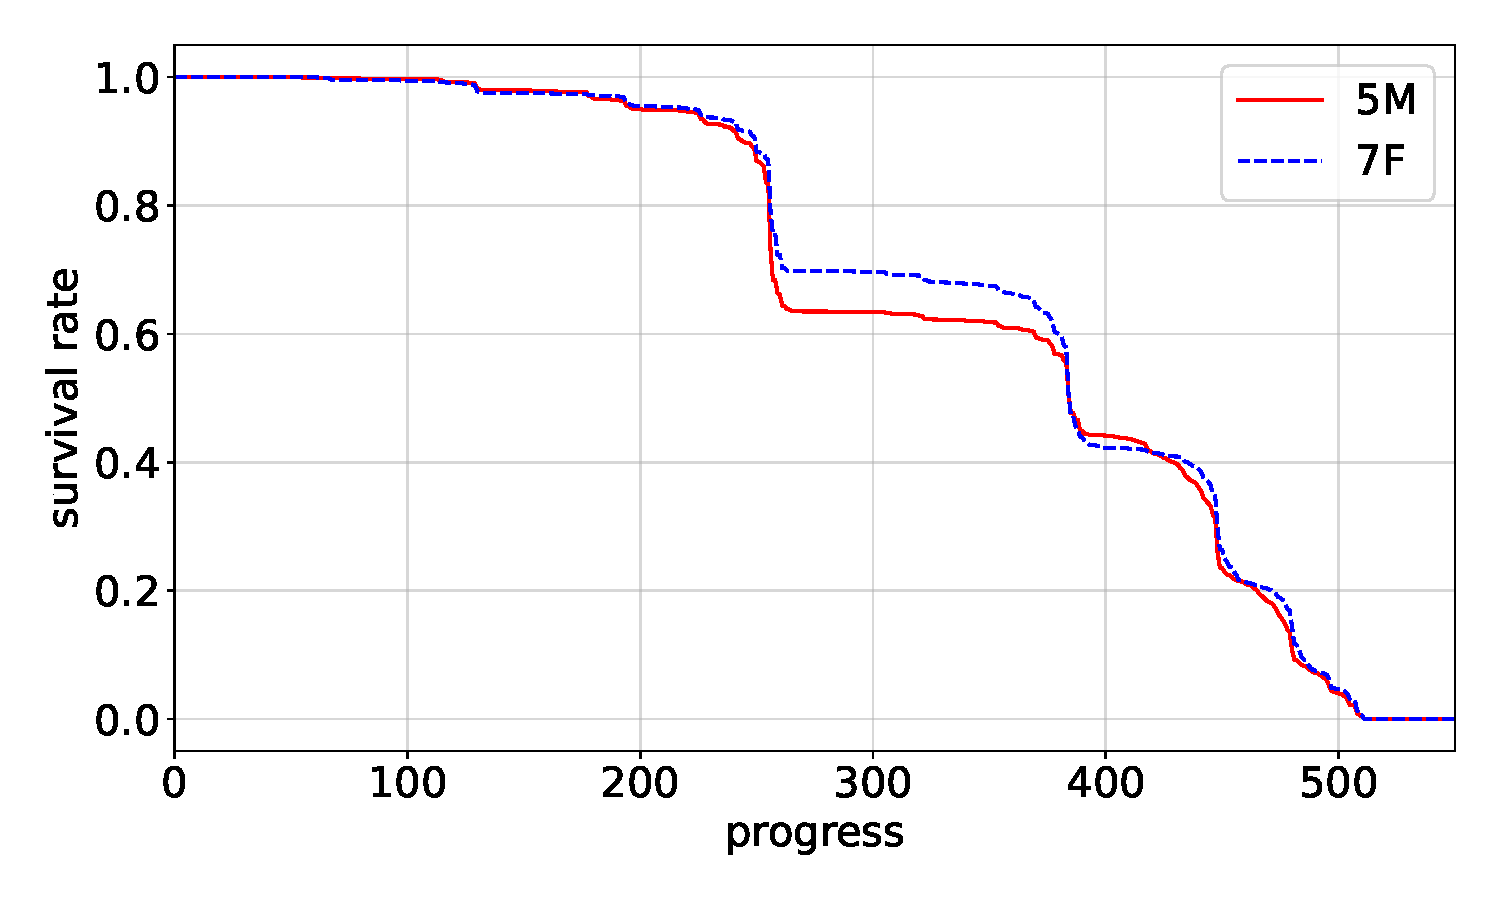
\includegraphics[width=\linewidth]{pdf/compare/EXP6_NT5M_and_NT7F/survival.pdf}
    \caption{生存率}
    \label{fig:EXP6_NT5M_and_NT7F_survival}
\end{subfigure}
\caption{5Mと7Fの比較結果(深さ6)}
\label{fig:EXP6_NT5M_and_NT7F_results}
\end{figure}

図\ref{fig:EXP6_NT4FとNT8M_results}と図\ref{fig:EXP6_NT5M_and_NT7F_results}は,
図\ref{fig:NT4F_and_NT8M_results}と図\ref{fig:NT5M_and_NT7F_results}のExpectimax探索深さ6を組み合わせたプレイヤである.
それぞれのスコアとしては向上していてそれは図\ref{fig:EXP6_NT4F_and_NT8M_error_abs_diff}と図\ref{fig:EXP6_NT5M_and_NT7F_error_abs}
の絶対誤差と図\ref{fig:EXP6_NT4F_and_NT8M_survival}と図\ref{fig:EXP6_NT5M_and_NT7F_survival}の生存率に現れている.
図\ref{fig:EXP6_NT4F_and_NT8M_accuracy}と図\ref{fig:EXP6_NT5M_and_NT7F_accuracy}の正確度はどちらも形はGreedyと似たような形になってる.